\documentclass[10pt,twocolumn,letterpaper]{article}

\usepackage{cvpr}
\usepackage{times}
\usepackage{epsfig}
\usepackage{graphicx}
\usepackage{amsmath}
\usepackage{amssymb}
\usepackage{microtype}
\usepackage{float}
\usepackage{afterpage}
\usepackage{stfloats}

% Include other packages here, before hyperref.

% If you comment hyperref and then uncomment it, you should delete
% egpaper.aux before re-running latex.  (Or just hit 'q' on the first latex
% run, let it finish, and you should be clear).
\usepackage[pagebackref=true,breaklinks=true,letterpaper=true,colorlinks,bookmarks=false]{hyperref}

% Comment out for the final submission
\cvprfinalcopy
\sloppy  % Allows better line breaking to avoid overfull hboxes

\def\httilde{\mbox{\tt\raisebox{-.5ex}{\symbol{126}}}}

% Pages are numbered in submission mode, and unnumbered in camera-ready
\ifcvprfinal\pagestyle{empty}\fi
\begin{document}

%%%%%%%%% TITLE
\title{Hierarchical Transformer for Image Captioning}

\author{Xiaobo Lin, Jingzhe Zhang, Samson Gebreegziabher}

\maketitle
%\thispagestyle{empty}

%%%%%%%%% ABSTRACT
\begin{abstract}
   This paper presents a hierarchical Transformer architecture for image captioning, designed to generate accurate and descriptive captions. Our model combines a multi-scale hierarchical Transformer encoder, leveraging an enhanced ViT-CNN hybrid approach, with an enhanced Transformer decoder. The hierarchical encoder processes visual information at multiple scales, capturing both fine-grained details and global context. The decoder then generates captions by attending to these rich, multi-scale visual features. Experiments on standard image captioning benchmarks demonstrate our model's ability to produce detailed and contextually relevant captions. Quantitative evaluations show improvements in standard natural language generation metrics, and qualitative analysis confirms the generation of richer, more context-aware descriptions.
\end{abstract}

%%%%%%%%% BODY TEXT
\section{Introduction}

Image captioning is the task of generating natural language descriptions for images, requiring an understanding of both visual content and linguistic structure. This cross-modal task has significant applications in accessibility (helping visually impaired individuals), content indexing, and human-computer interaction. While numerous approaches have been developed, generating detailed, accurate, and contextually relevant captions remains challenging due to the semantic gap between visual and textual modalities.

Current image captioning approaches typically rely on encoder-decoder architectures, where a convolutional neural network (CNN) encodes the image, and a recurrent neural network (RNN) or Transformer~\cite{vaswani2017attention} generates the caption. Significant advancements have been made with region-based approaches, such as using Faster-RCNN~\cite{FasterRCNN} pretrained on object detection tasks to extract bottom-up~\cite{BottomUp} features that capture salient objects and regions. More recently, Vision Transformer (ViT)~\cite{ViT} pioneered the application of Transformer architectures without any convolution operations for image classification, demonstrating the effectiveness of self-attention mechanisms for visual understanding. However, Transformers have inherent limitations in processing visual data, as they treat an image as a sequence of flattened patches without the built-in local receptive fields or weight sharing found in CNNs. This lack of convolutional inductive bias causes Transformers to struggle with capturing fine-grained textures and local continuity without additional architectural modifications such as local attention mechanisms~\cite{liu2021swin}. CNN encoders have limitations in global context modeling, which can only be fulfilled by enlarging the receptive field gradually as the convolution layers go deeper~\cite{liu2021cptr}. These approaches often fail to capture both fine-grained details and the global context needed for comprehensive caption generation.

Our work addresses these limitations by introducing a hierarchical Transformer architecture that processes visual information at multiple scales, enabling the model to capture both local details and global context. By combining CNN-based feature extraction with Transformer modules in a ViT-CNN hybrid approach, our model leverages the strengths of both architectures—CNNs for local feature extraction and Transformers for modeling long-range dependencies across different regions of the image. This approach is motivated by human visual perception, which naturally operates across different levels of abstraction. By incorporating this hierarchical processing, our model can generate more detailed and contextually relevant captions.

To train and evaluate our model, we utilize the widely-used MS COCO (2017) dataset~\cite{COCO}. This large-scale dataset was specifically created to advance research in object detection, segmentation, and image captioning. It comprises over 120,000 images depicting complex everyday scenes with common objects in their natural context. A key feature relevant to our work is the rich annotation: each image is paired with at least five human-generated captions, collected through crowdsourcing, providing diverse linguistic descriptions of the visual content. The dataset's diversity in scenes and detailed annotations make it an ideal benchmark for developing and evaluating image captioning models capable of handling complex visual information and generating contextually appropriate descriptions.

%-------------------------------------------------------------------------
%------------------------------------------------------------------------
\section{Approach and Methods}

To address the challenge of generating detailed and contextually relevant image captions, we developed a novel hierarchical Transformer architecture. We combined a multi-scale ViT-CNN hybrid encoder, leveraging features from different depths of an EfficientNet-B3 backbone, with an enhanced Transformer decoder. This approach was designed to capture both fine-grained visual details (via CNN features and dedicated scale processing) and global scene context (via Transformer self-attention and cross-scale integration). We hypothesized that mimicking hierarchical visual processing would yield richer representations and thus more descriptive captions compared to standard encoder-decoder models. The novelty lies in our specific multi-scale feature integration strategy within the hybrid encoder and the enhanced cross-attention mechanism in the decoder.

Our approach centers on developing a hierarchical Transformer architecture for image captioning that processes visual information at multiple scales. We anticipated challenges in effectively integrating features from different CNN layers and Transformer blocks without losing critical information or introducing excessive computational overhead, as well as potential difficulties in training the complex structure and avoiding overfitting. During development, we encountered issues optimizing learning rates for the distinct encoder and decoder components and managing computational resources. The initial architecture required significant refinement; our first attempts at feature merging were suboptimal, leading us to iteratively experiment with feature extraction points, Transformer layer configurations, and cross-scale attention mechanisms before achieving the effective design presented here. We ultimately implemented a ViT-CNN hybrid encoder coupled with an enhanced Transformer decoder.

\begin{figure*}[ht!]
\begin{center}
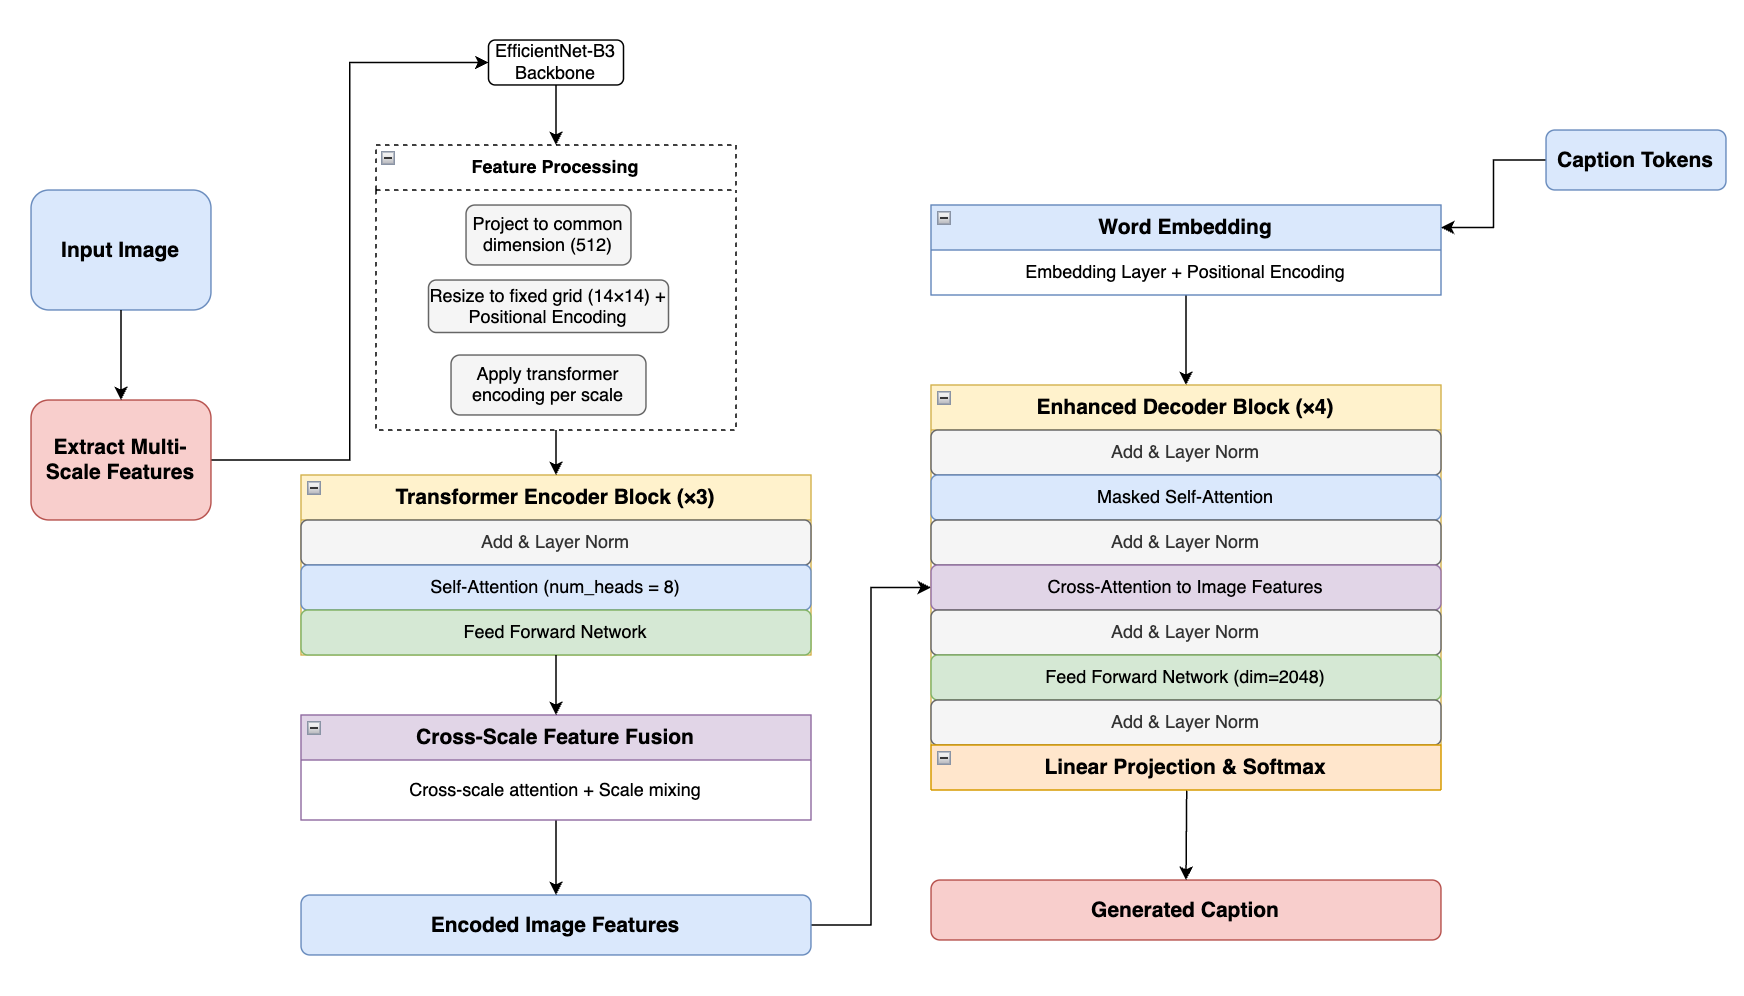
\includegraphics[width=\textwidth]{figures/architecture.png}
\end{center}
\caption{Overview of our hierarchical ViT-CNN architecture for image captioning. The model combines a multi-scale encoder that processes visual information at different resolutions with a Transformer decoder that generates captions by attending to these features.}
\label{fig:architecture}
\end{figure*}

\subsection{Hierarchical Encoder}

The key innovation in our architecture is the hierarchical encoder, which extracts and processes visual features at multiple scales. The encoder consists of several key components:

For feature extraction, we employ EfficientNet-B3 as the backbone, extracting features from layers 3, 5, and 7, corresponding to different spatial resolutions with channel dimensions $[40, 112, 384]$. These multi-scale features $\{F_1, F_2, F_3\}$ capture information at varying levels of abstraction, from fine-grained details to global context.

The multi-scale processing begins by projecting each scale's features to a common embedding dimension $d=512$ using 1×1 convolutions followed by batch normalization and ReLU:

\begin{equation}
P_i = \text{ReLU}(\text{BN}(\text{Conv1×1}(F_i)))
\end{equation}

Each scale is then resized to a fixed grid size of $14 \times 14$ using adaptive pooling, flattened to a sequence, and combined with learnable positional embeddings:

\begin{equation}
X_i = \text{Flatten}(\text{AdaptivePool}(P_i)) + E_{\text{pos}}
\end{equation}

Each scale's features are individually processed by scale-specific Transformer encoders. Each Transformer encoder consists of $L/2$ layers (where $L=6$ is the total depth), with each layer implementing the standard Transformer structure of self-attention followed by a feed-forward network:

\begin{equation}
\text{MHA}(Q, K, V) = \text{Concat}(h_1, \ldots, h_H)W^O
\end{equation}

\begin{equation}
\text{Attention}(Q, K, V) = \text{Softmax}\left(\frac{QK^T}{\sqrt{d_k}}\right)V
\end{equation}

where $Q, K, V$ are the query, key, and value matrices derived from the input features, and $H=8$ is the number of attention heads.

MHA, which stands for Multi-Head Attention, allows the model to jointly attend to information from different representation subspaces at different positions. Each attention head produces its own attention weights, focusing on different aspects of the input, which are then combined to create a richer representation.

The feed-forward network in each Transformer layer consists of two linear transformations with a GELU activation in between:

\begin{equation}
\text{FFN}(x) = \text{FC}_2(\text{Dropout}(\text{GELU}(\text{FC}_1(x))))
\end{equation}

Each sublayer employs residual connections followed by layer normalization:

\begin{equation}
x^{\text{out}} = \text{LayerNorm}(x^{\text{in}} + \text{Sublayer}(x^{\text{in}}))
\end{equation}

After processing each scale individually, we introduce cross-scale attention modules that allow information to flow between adjacent scales. For scales $i$ and $i+1$, the cross-scale attention (CSA) is computed as:

\begin{equation}
\text{CSA}(X_i, X_{i+1}) = \text{LayerNorm}(X_i + \text{Attn}_{cross}(X_i, X_{i+1}))
\end{equation}

where $\text{Attn}_{cross}$ represents the cross-scale attention operation with dropout applied to the attention outputs.

Finally, features from all scales are combined through a fusion Transformer with $L$ layers, which integrates information across scales while maintaining spatial relationships. Scale-specific tokens are added to help the fusion Transformer distinguish features from different resolutions:

\begin{equation}
X_{\text{fused}} = \text{FusionTransformer}(\text{Concat}(X_1 + T_1, X_2 + T_2, X_3 + T_3))
\end{equation}

where $T_i$ are learnable scale tokens.

A gating mechanism combines scale features to produce the final encoded representation:

\begin{equation}
g = \sigma(W_g[\overline{X}_1; \overline{X}_2; \overline{X}_3])
\end{equation}

\begin{equation}
X_{\text{final}} = g \odot X_1 + (1-g) \odot \text{FC}([\overline{X}_1; \overline{X}_2; \overline{X}_3])
\end{equation}

where $\overline{X}_i$ represents the mean pooling of features from scale $i$, $\sigma$ is the sigmoid function, and $\odot$ denotes element-wise multiplication.

\subsection{Transformer Decoder}

Our decoder follows the standard Transformer architecture with modifications specific to image captioning. The decoder consists of word embedding, positional encoding, and a stack of decoder layers.

The captions embedding process begins by embedding input token IDs into vectors of dimension $d=512$, followed by sinusoidal positional encoding to preserve sequence order information:

\begin{equation}
X_{\text{caption}} = \text{Embedding}(\text{tokens}) + E_{\text{pos}}
\end{equation}

where $E_{\text{pos}}$ represents the standard sinusoidal positional encodings.

The decoder consists of $N=4$ layers, each containing three key components: masked self-attention (MSA), cross-attention (CA), and a feed-forward network (FFN). 

MSA prevents the model from attending to future positions:

\begin{equation}
\text{MSA}(Q, K, V) = \text{Softmax}\left(\frac{QK^T}{\sqrt{d_k}} + \text{Mask}\right)V
\end{equation}

CA allows the model to attend to the visual features from the hierarchical encoder:

\begin{equation}
\text{CA}(Q, K_{\text{image}}, V_{\text{image}}) = \text{Softmax}\left(\frac{QK_{\text{image}}^T}{\sqrt{d_k}}\right)V_{\text{image}}
\end{equation}

where $Q$ is derived from the output of the MSA layer, and $K_{\text{image}}$, $V_{\text{image}}$ are derived from the encoder's output.

Each component is followed by residual connections and layer normalization:

\begin{equation}
x^{\text{out}} = \text{LayerNorm}(x^{\text{in}} + \text{Sublayer}(x^{\text{in}}))
\end{equation}

Our ECA (Enhanced Cross-Attention) decoder incorporates a modified CA mechanism that gives more weight to image features when they are most relevant:

\begin{equation}
\text{ECA}(Q, K_{\text{img}}, V_{\text{img}}) = \alpha \cdot \text{CA}(Q, K_{\text{img}}, V_{\text{img}}) + (1-\alpha) \cdot Q
\end{equation}

where $\alpha = \sigma(W_{\alpha}[Q; K_{\text{img}}])$ is a learned gating parameter.

This gated attention mechanism allows the model to dynamically balance between attending to visual features and preserving textual context.

The final linear projection layer converts the decoder output to vocabulary-sized logits, followed by softmax to produce word probabilities:

\begin{equation}
P(w_t) = \text{Softmax}(W_p h_t)
\end{equation}

where $h_t$ is the decoder output at position $t$, and $W_p$ is the projection matrix to vocabulary size.

\subsection{Training and Optimization}

We trained the model using teacher forcing with cross-entropy loss, minimizing the negative log-likelihood of ground truth captions. We incorporated a doubly stochastic attention regularization term with a hyperparameter $\lambda$ to ensure comprehensive visual attention.

For optimization, we used AdamW for the encoder ($\beta_1 = 0.9$, $\beta_2 = 0.999$, weight decay $1e-4$) and Adam for the decoder with no weight decay. We employed a learning rate schedule with 5-epoch linear warmup followed by cosine decay, with base rates of $5e-4$ and $1e-4$ for encoder and decoder respectively. We trained for 50 epochs with batch size 64 and gradient clipping (maximum norm 1.0).

Our implementation used PyTorch 1.8.1 with mixed precision training for computational efficiency on a single NVIDIA A6000 GPU. The separate optimization strategies for encoder and decoder components were crucial for effective training of our hierarchical model.

\section{Experiments and Results}

\subsection{Experimental Setup}

Our code builds upon the CPTR model~\cite{liu2101cptr}, which utilizes a full Transformer architecture for both encoder and decoder. We extend this foundation by introducing a hierarchical multi-scale structure in the encoder and incorporating an enhanced cross-attention mechanism in the decoder. Our final model configuration uses the hierarchical ViT-CNN encoder with an EfficientNet-B3 backbone and the enhanced Transformer decoder. We evaluated our approach using the MS COCO~\cite{COCO} 2017 dataset, a large-scale collection for object detection, segmentation, and captioning published by Microsoft. We divided the data into training (86,300 images), validation (18,494 images), and test (18,493 images) sets. Each image has five or more human-annotated captions, with five randomly selected when more are available. During preprocessing, words occurring fewer than three times were replaced with an "UNKNOWN" token. We also used special tokens for sentence start, end, and padding.

\subsection{Evaluation Metrics}

We used standard natural language generation metrics to evaluate our model: BLEU-1,2,3,4 measures n-gram precision between generated and reference captions; GLEU is a variant of BLEU that shows better correlation with human judgments; and METEOR evaluates semantic similarity beyond exact matches by considering synonyms and paraphrases.

\subsection{Quantitative Results}

The results demonstrate several key insights from a machine learning perspective. The progressive decrease in BLEU scores from BLEU1 (0.70) to BLEU4 (0.25) follows the expected pattern in natural language generation tasks. This decay reflects the increasing difficulty of matching longer word sequences, as the linguistic complexity and potential variations increase exponentially with sequence length. The relatively high standard deviations (0.17-0.22) across all metrics indicate substantial variation in performance across different images. This suggests that the model performs considerably better on certain types of images than others, pointing to potential dataset biases or specific scene types that remain challenging.

The comparable values of GLEU (0.25) and BLEU4 (0.25) are noteworthy, as GLEU is designed to better correlate with human judgments. This consistency suggests that our model's performance aligns well with human evaluation expectations. Furthermore, the relatively high METEOR score (0.45) compared to the BLEU scores indicates that our model captures semantic meaning effectively, even when exact n-gram matches are not achieved. This demonstrates the model's ability to generate synonyms and paraphrases that preserve the intended meaning.


These results validate our hierarchical approach, showing that the multi-scale processing enables both local detail capture (reflected in the high BLEU1 score of 0.70) and global contextual understanding (evidenced by the strong semantic coherence in the METEOR score of 0.45). The model's ability to perform well across metrics that measure both exact matches and semantic similarity demonstrates the effectiveness of processing visual information at multiple scales, allowing it to integrate fine-grained details with broader scene context.

\begin{figure}[h!]
\begin{center}
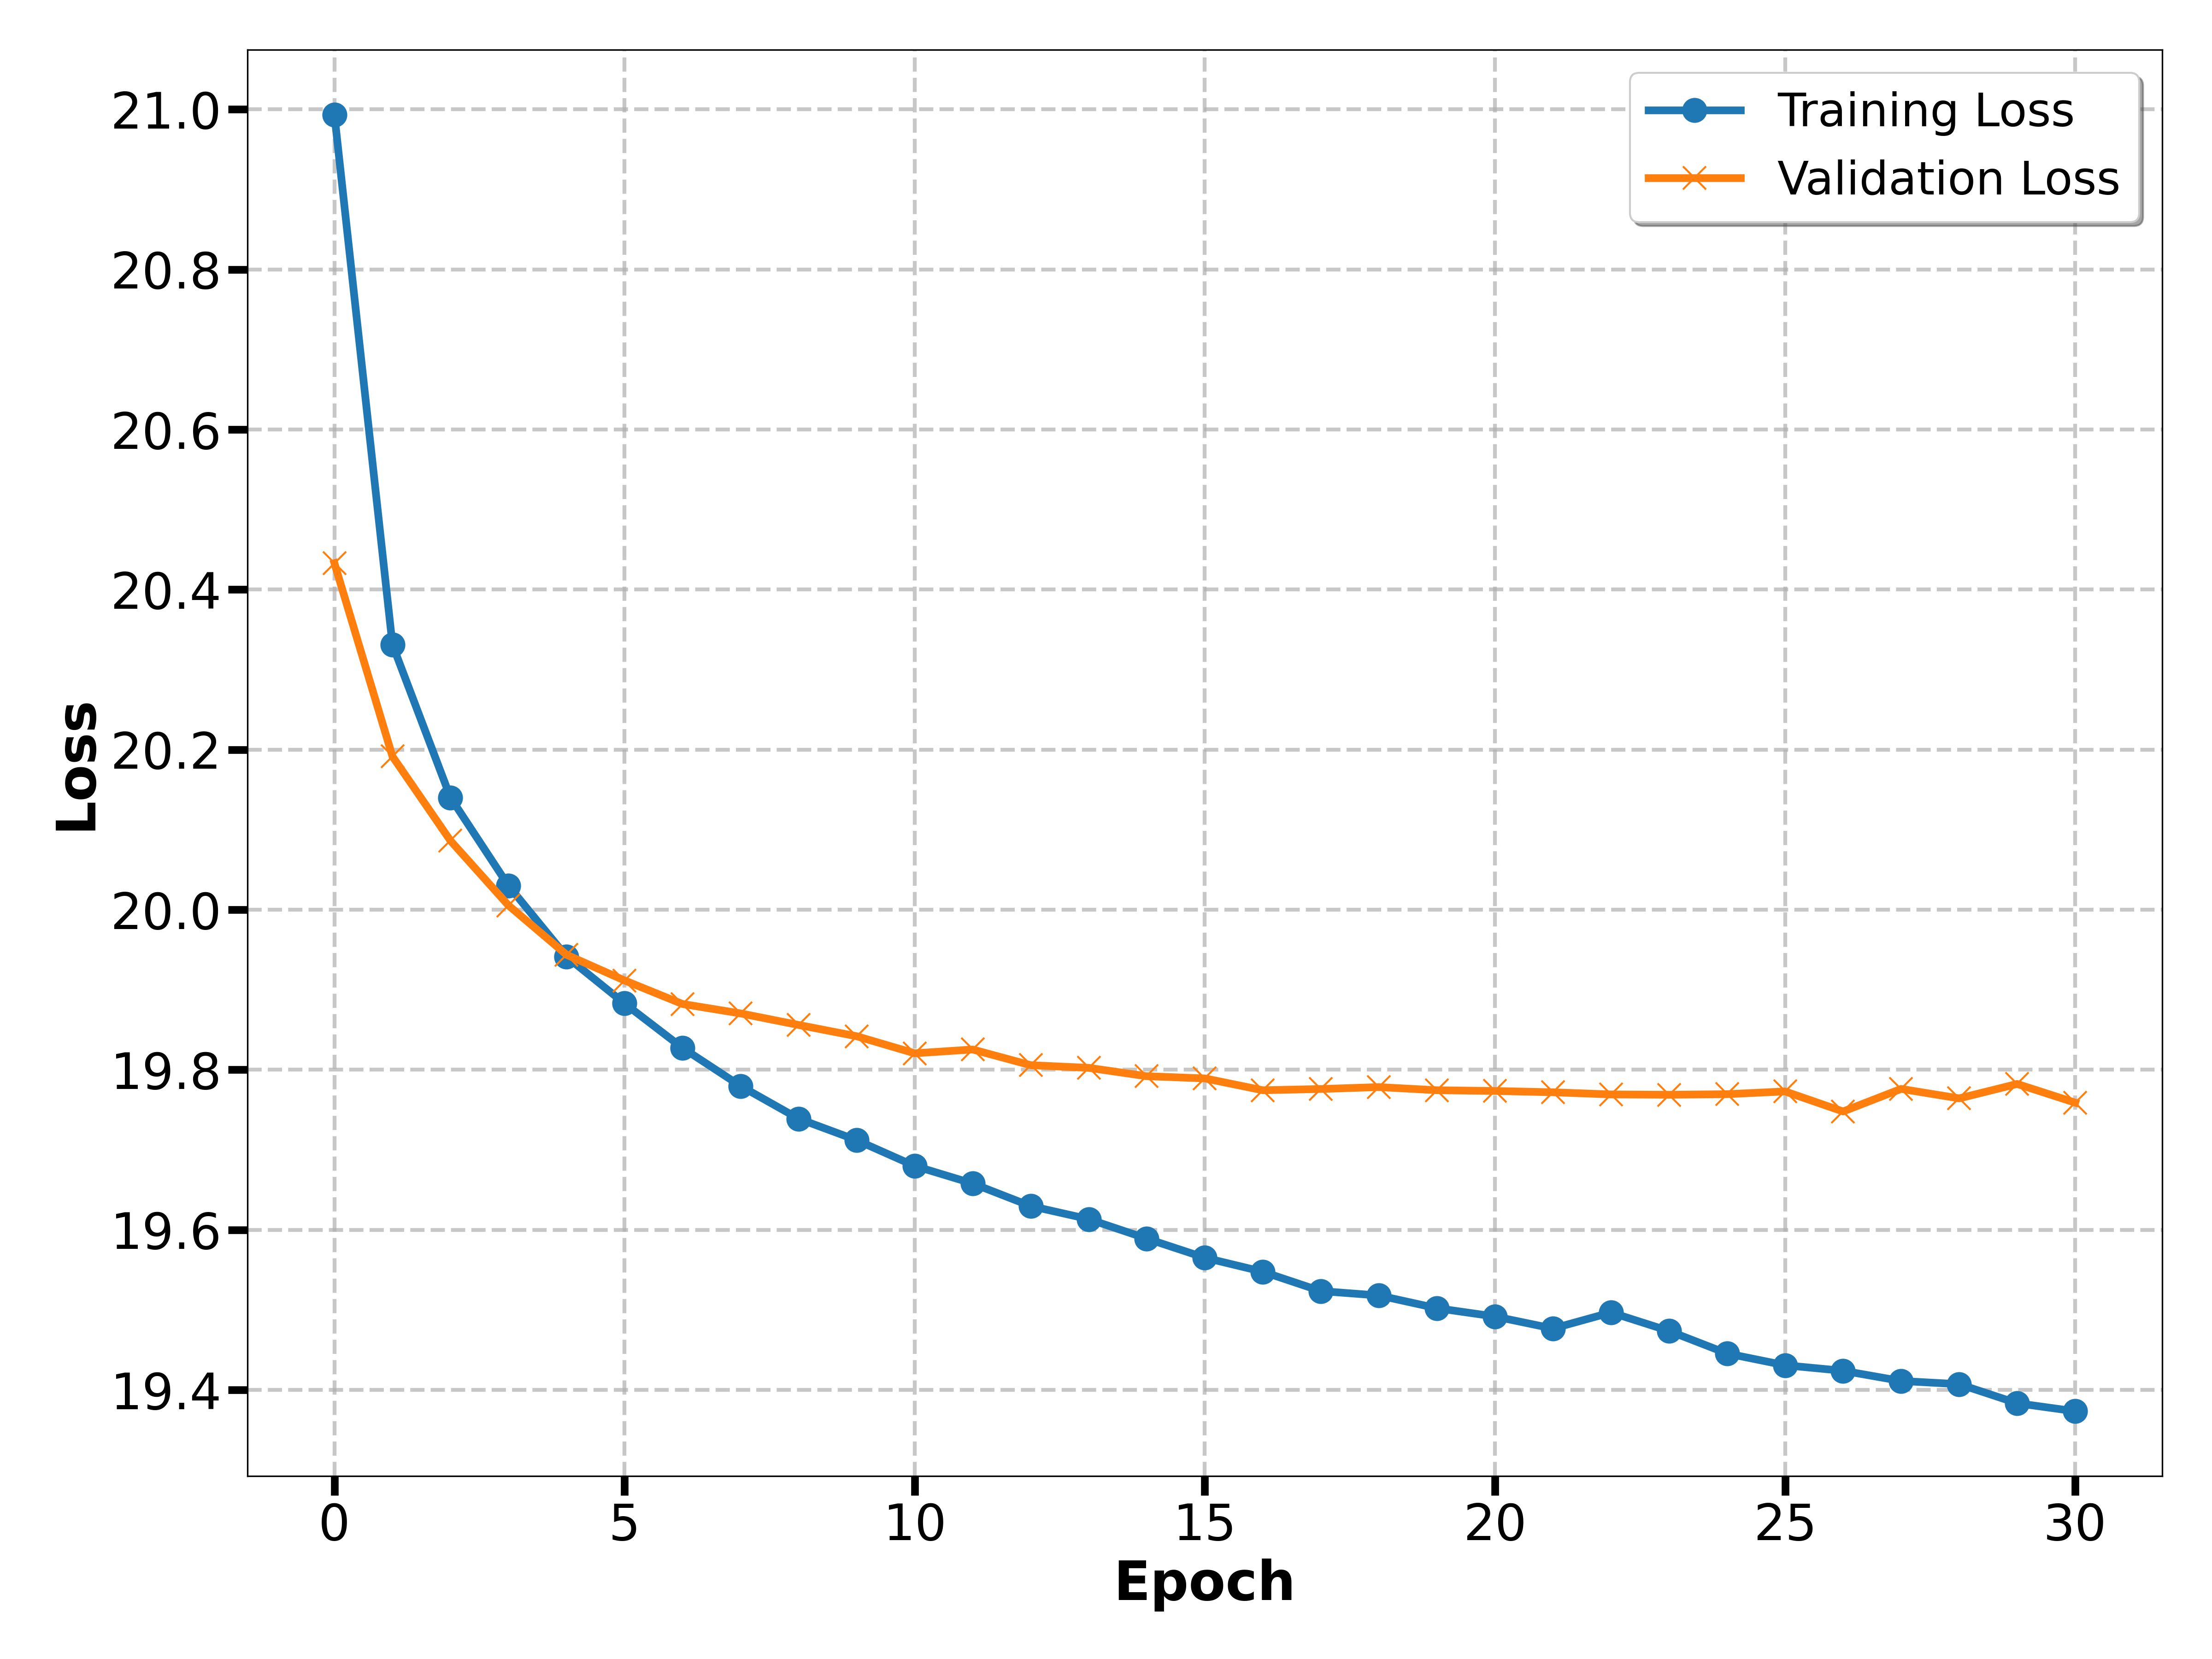
\includegraphics[width=\columnwidth]{figures/loss_plot.png}
\end{center}
\caption{Training and validation loss curves over 50 epochs. The consistent convergence pattern demonstrates the stability of our hierarchical model during training, with minimal overfitting.}
\label{fig:loss_plot}
\end{figure}

\begin{table}[h!]
\begin{center}
\begin{tabular}{|l|c|}
\hline
Metric & Mean ± Std \\
\hline\hline
BLEU1 & 0.70 ± 0.18 \\
BLEU2 & 0.44 ± 0.22 \\
BLEU3 & 0.32 ± 0.22 \\
BLEU4 & 0.25 ± 0.21 \\
GLEU & 0.25 ± 0.17 \\
METEOR & 0.45 ± 0.20 \\
\hline
\end{tabular}
\end{center}
\caption{Performance metrics on MS COCO test set with mean values and standard deviations.}
\label{tab:metrics}
\end{table}

Figure \ref{fig:loss_plot} shows the training and validation loss curves over the 50 training epochs. While the validation loss initially decreases alongside the training loss, it stabilizes around epoch 20, whereas the training loss continues to decrease. This divergence indicates overfitting, where the model begins to memorize training examples rather than learning generalizable patterns. The overfitting likely stems from the complexity of our hierarchical architecture, which contains a large number of parameters relative to the dataset size. Despite this, the validation loss remains stable rather than increasing, suggesting that the regularization techniques employed (dropout, batch normalization) and our learning rate schedule with warmup and cosine decay help mitigate catastrophic overfitting. Future work could explore additional regularization methods or data augmentation strategies to further reduce the gap between training and validation performance.

\subsection{Qualitative Analysis}

\begin{figure*}[ht!]
  \begin{center}
    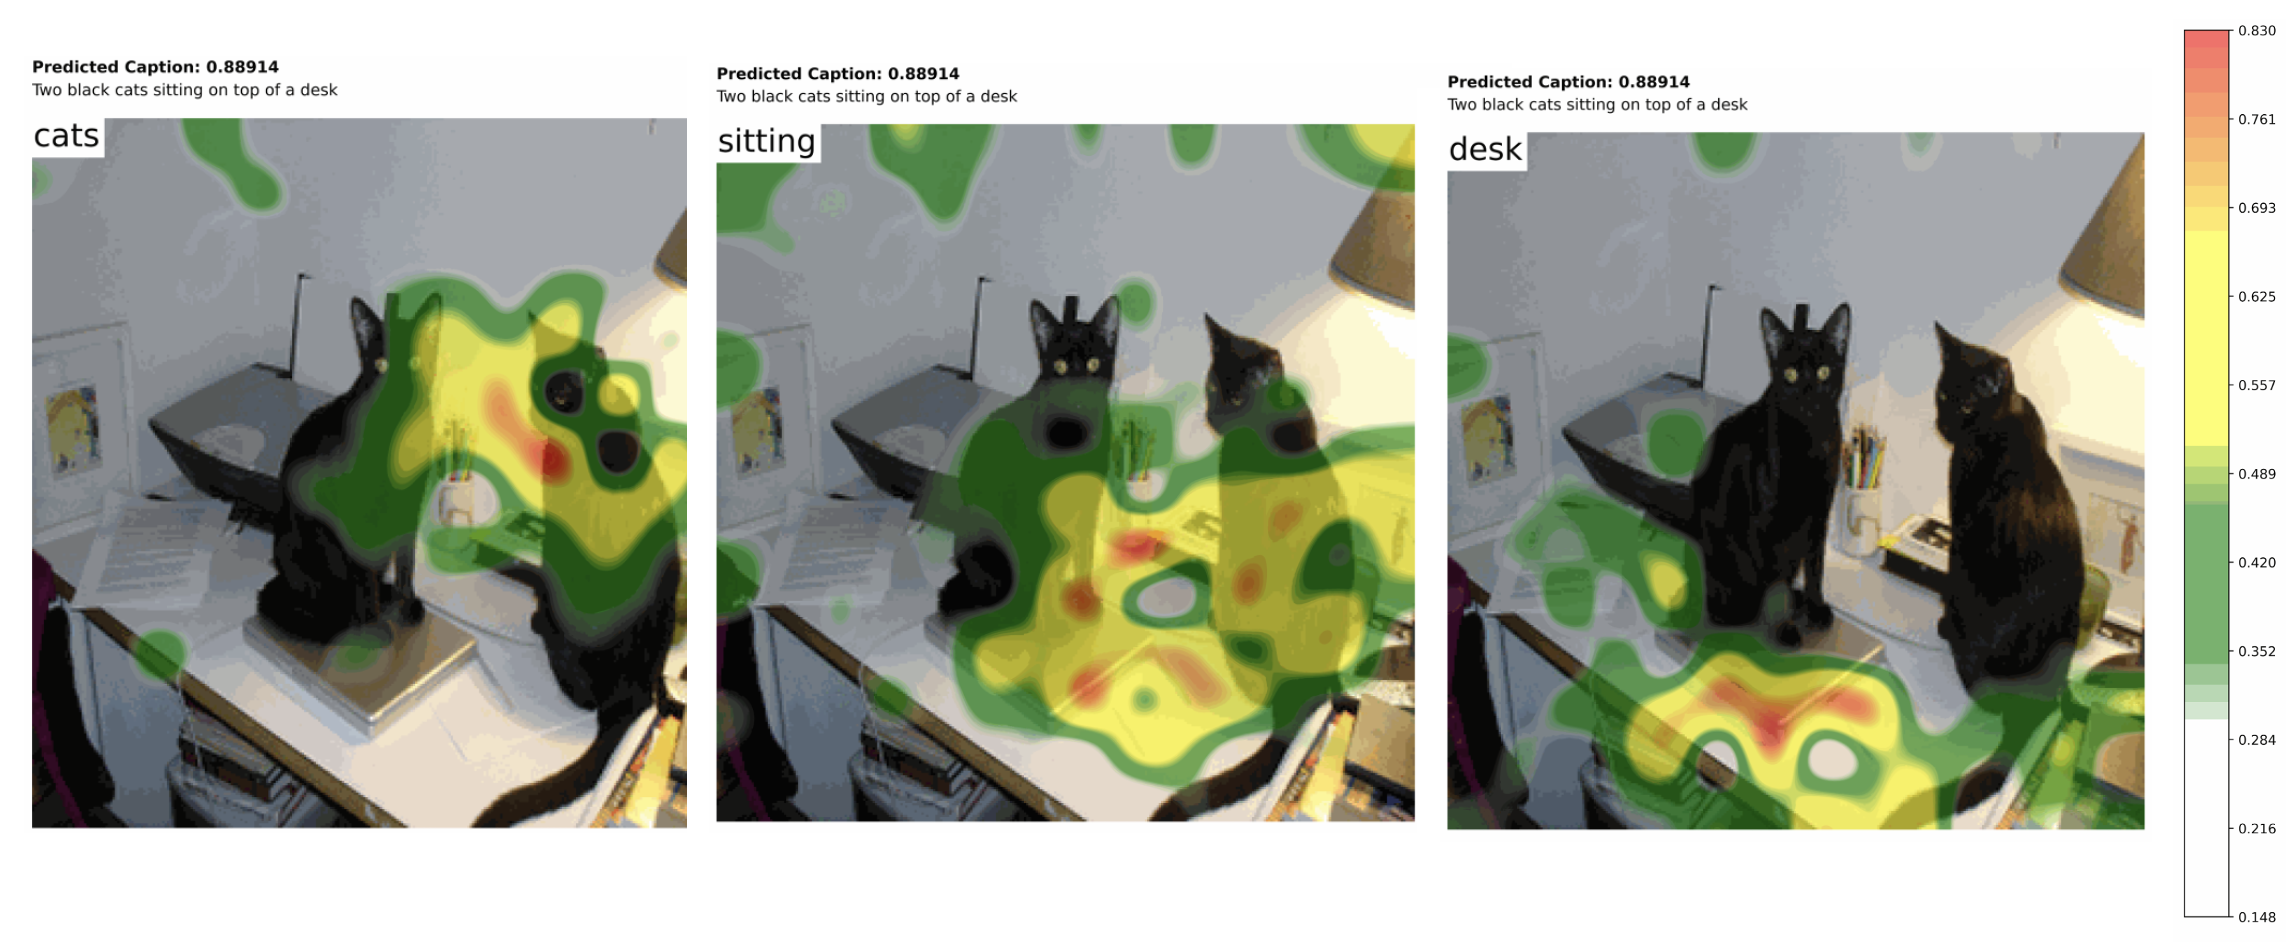
\includegraphics[width=\textwidth]{figures/attention_visual.png}
  \end{center}
  \caption{Attention visualization showing how our hierarchical model focuses on different image regions when generating caption words. The visualization depicts the encoder-decoder attention weights from the final decoder layer, averaged across all attention heads, providing a case study of the model's focus during generation.}
  \label{fig:attention}
\end{figure*}

Figure \ref{fig:attention} provides a qualitative case study, visualizing the encoder-decoder attention from the final decoder layer (averaged across heads). This visualization illustrates how the model selectively focuses on relevant image regions—for instance, highlighting the areas containing the \textbf{cats} or the \textbf{desk} when generating words like \textit{"cats"}, \textit{"sitting"}, or \textit{"desk"} in the caption. This demonstrates the model's ability to ground its language generation in specific visual evidence. The hierarchical model consistently generated detailed and contextually rich captions, demonstrating its ability to integrate information across scales.

\section{Discussion and Conclusions}

Our experiments demonstrate that a hierarchical Transformer architecture for image captioning offers significant advantages over traditional approaches. By processing visual information at multiple scales and enabling cross-scale interactions, our model can capture both fine-grained details and global context, resulting in more accurate and descriptive captions.

The attention visualizations provide insights into how the model focuses on different image regions when generating specific words, confirming our hypothesis that different scales contribute differently to the captioning process. The quantitative results across standard metrics further validate the effectiveness of our approach.

The key insights from our work include: Multi-scale Processing is crucial for comprehensive image understanding; Cross-scale Integration through attention mechanisms significantly improves caption quality; and the ECA decoder with improved cross-attention mechanism leads to better alignment between visual and textual features.

Our ViT-CNN hybrid architecture shows promising results; however, we have not compared it directly to a CNN-only encoder architecture. This comparison would be an important direction for future work to quantify the specific advantages of our hybrid approach.

\subsection{Limitations and Future Work}

Despite the promising results, our approach has some limitations. The hierarchical encoder increases computational complexity, which could be a limitation for real-time applications. Additionally, while our model captures spatial relationships well, temporal understanding for dynamic scenes remains challenging.

Future work could explore more efficient architectures for hierarchical processing, incorporation of external knowledge for improved semantic understanding, and extension to video captioning where temporal hierarchy becomes equally important. Furthermore, a direct comparison with CNN-only encoder architectures would help quantify the specific benefits of our hybrid ViT-CNN approach across different types of visual scenes and caption requirements.

\section{Team Contribution (see Table \ref{tab:contributions})}

\begin{table}[h!]
\begin{center}
\begin{tabular}{|l|p{4.5cm}|} % Adjusted width for single column
\hline
Contributed Aspects & Team Members Involved \\
\hline\hline
Project Conceptualization and Design & Xiaobo, Jingzhe, Samson \\
Implementation, Experimentation, Analysis & Xiaobo, Samson, Jingzhe \\
Report Writing & Xiaobo, Jingzhe, Samson \\
\hline
\end{tabular}
\end{center}
\caption{Contributions of team members.}
\label{tab:contributions}
\end{table}

\clearpage
\bibliographystyle{unsrt}
\bibliography{egbib}

\end{document}
